\clearpage
\begin{explanationbox}
\textbf{从初中熟悉的几何开始：为什么共焦之后能求交点？}

取焦点 $F_1(-c,0),F_2(c,0)$，在第一象限设一个交点 $P=(X,Y)$。
\textbf{先不写两个二次方程}，只观察同一对距离
$r_1=PF_1$、$r_2=PF_2$：
\[
r_1+r_2=2a_E\quad(\text{椭圆定义}),\qquad
r_1-r_2=2a_H\quad(\text{双曲线右支定义}).
\]
为什么是\emph{同一对}距离？因为两曲线共用的不是一条坐标轴，
而是\textbf{完全相同的两点} $F_1,F_2$；椭圆给距离的\emph{和}，双曲线给\emph{差}。
解这个初中二元一次方程组：
\[
\boxed{r_1=a_E+a_H},\qquad\boxed{r_2=a_E-a_H}.
\]
\textbf{几何解释：}$a_E$ 是两距离的平均值，$a_H$ 是离平均值的偏差。
条件 $a_E>c>a_H>0$ 保证
$\lvert r_1-r_2\rvert=2a_H<2c<2a_E=r_1+r_2$，
即三边可以构成一个\textbf{非退化三角形}，上、下各有一点。
关于 $y$ 轴再反射，正好得到另外两个点。

\textbf{结论的形状先于数字：}圆锥曲线方程都含 $x^2,y^2$，
故点关于 $x$、$y$ 轴对称；只需求第一象限的 $X,Y>0$，
便立即得到 $(\pm X,\pm Y)$ 四点。
\end{explanationbox}

\clearpage
\begin{explanationbox}
\textbf{为什么「焦半径平方相减」会直接给出横坐标？}

\begin{center}
% Exact model: a_E=5, c=3, a_H=2; X=10/3, Y=4 sqrt(5)/3.
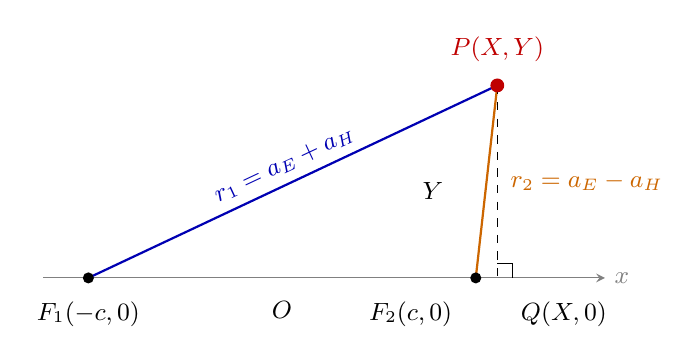
\begin{tikzpicture}[x=.82cm,y=.82cm,>=stealth,font=\small]
\coordinate (L) at (-3,0); \coordinate (R) at (3,0);
\coordinate (P) at (10/3,{4*sqrt(5)/3}); \coordinate (Q) at (10/3,0);
\draw[->,gray] (-3.7,0)--(5,0) node[right] {$x$};
\draw[blue!70!black,thick] (L)--(P) node[midway,above,sloped] {$r_1=a_E+a_H$};
\draw[orange!80!black,thick] (R)--(P) node[midway,right=5pt] {$r_2=a_E-a_H$};
\draw[dashed] (P)--(Q) node[pos=.55,left=16pt] {$Y$};
\draw (10/3,.23)--({10/3+.23},.23)--({10/3+.23},0);
\fill (L) circle (2pt) node[below=5pt] {$F_1(-c,0)$};
\fill (R) circle (2pt) node[below left=5pt] {$F_2(c,0)$};
\fill[red!75!black] (P) circle (2.5pt) node[above=5pt] {$P(X,Y)$};
\node[below right=5pt] at (Q) {$Q(X,0)$};
\node[below=5pt] at (0,0) {$O$};
\end{tikzpicture}


{\small 共用高度 $Y$，相减便消去 $Y^2$；$Q$ 不必位于两焦点之间。}
\end{center}
图中两个直角三角形给出
\[
PF_1^2=(X+c)^2+Y^2,\qquad PF_2^2=(X-c)^2+Y^2.
\]
两式\textbf{相减}，相同的 $Y^2$ 恰好消去：
\[
PF_1^2-PF_2^2=(X+c)^2-(X-c)^2=4cX.
\]
几何意义：两个焦点左右对称，距它们的\emph{平方差}
只反映点在焦点轴方向偏向哪边，因此直接确定 $X$。
由焦半径 $a_E\pm a_H$ 同时得
\[
PF_1^2-PF_2^2=(a_E+a_H)^2-(a_E-a_H)^2=4a_Ea_H.
\]
两边相等，便有 $X=a_Ea_H/c$。

\textbf{那为什么下一步要「相加」？}
\[
\frac{PF_1^2+PF_2^2}{2}=X^2+Y^2+c^2=a_E^2+a_H^2.
\]
相加消去的是\emph{方向项} $\pm2cX$，得到点到原点的距离平方
$X^2+Y^2$；由此推出 $Y^2$。
\[
\begin{aligned}
Y^2&=a_E^2+a_H^2-c^2-\frac{a_E^2a_H^2}{c^2}\\
&=\frac{(a_E^2-c^2)(c^2-a_H^2)}{c^2}
=\frac{b_E^2b_H^2}{c^2}.
\end{aligned}
\]
\textbf{两种运算不是口诀：}相减消去高度、找横坐标；
相加消去左右差异、找离原点的距离，再确定高度。
\end{explanationbox}

\clearpage
\begin{explanationbox}
\textbf{从标准方程看：为什么令 $u=x^2,v=y^2$ 最省心？}

和一般二次方程不同，这里 $x$、$y$ 不以一次项出现；
所以直接把 $u=x^2,v=y^2$ 当作两个未知数，
把两条二次曲线变成\textbf{两条关于 $u,v$ 的直线}：
\[
\frac{u}{a_E^2}+\frac{v}{b_E^2}=1,\qquad
\frac{u}{a_H^2}-\frac{v}{b_H^2}=1.
\]
解出唯一的 $u,v$ 后，它们都为正，
因此每一个平方都能开正、负两种根：
\[
u=X^2>0,\quad v=Y^2>0
\quad\Longrightarrow\quad (x,y)=(\pm X,\pm Y).
\]
\textbf{为什么恰为四点、不是更多？}上述线性方程组的行列式
$-1/(a_E^2b_H^2)-1/(a_H^2b_E^2)<0$，故 $u,v$ 只有\emph{一组}；
每个正平方给两个符号，恰好 $2\times2=4$ 个不同的点。
不存在第五个点，也不存在只有两个实交点的情况。

\textbf{尺度与形状分开记：}令 $e_E=c/a_E$、$e_H=c/a_H$，则
\[
\frac{X}{a_E}=\frac{a_H}{c}=\frac1{e_H},\qquad
\frac{Y}{b_E}=\frac{b_H}{c}=\sqrt{1-\frac1{e_H^2}}.
\]
椭圆沿 $x,y$ 分别缩放成单位圆后，这四点的\emph{归一化位置}
只由双曲线离心率 $e_H$ 决定；再按椭圆轴长拉伸回原坐标，得到实际交点。
\end{explanationbox}

\clearpage
\begin{explanationbox}
\textbf{几何延伸：为什么两曲线在四个交点处互相垂直？}

\begin{center}
% At P=(2,3), slopes -1/2 and 2. Same scale on both axes.
\begin{tikzpicture}[x=.75cm,y=.75cm,>=stealth,font=\small]
\draw[->,gray] (-2.7,0)--(5.6,0) node[right] {$x$};
\draw[blue!70!black,thick,domain=15:105,samples=70,variable=\t]
 plot ({4*cos(\t)},{sqrt(12)*sin(\t)});
\draw[orange!80!black,thick,domain=.3:4.9,samples=70,variable=\t]
 plot ({sqrt(1+\t*\t/3)},\t);
\draw[blue!70!black,dashed] (-.5,4.25)--(5.2,1.4) node[right] {$k_E=-1/2$};
\draw[orange!80!black,dashed] (.6,.2)--(3,5) node[above right] {$k_H=2$};
\draw[gray] (-2,0)--(2,3)--(2,0);
\draw[thick] (2.358,2.821)--(2.537,3.179)--(2.179,3.358);
\fill[red!75!black] (2,3) circle (2.5pt) node[above left=5pt] {$P$};
\fill (-2,0) circle (2pt) node[below] {$F_1$};
\fill (2,0) circle (2pt) node[below] {$F_2$};
\node at (0,-1.3) {切线夹角 $90^\circ$，焦角 $\cos\theta=3/5$};
\end{tikzpicture}


{\small 同一交点处，切线相互垂直；灰色焦半径的夹角不是直角。}
\end{center}
在例图的 $P=(2,3)$ 处，$k_E=-1/2$、$k_H=2$，故两切线垂直。
一般交点也满足 $k_Ek_H=-1$，完整推导见后面的推论证明。

\textbf{直觉：}椭圆是「两焦点距离\emph{和}固定」的等值线，
双曲线是「两焦点距离\emph{差}固定」的等值线；
二者的法向量分别与两条单位焦半径向量的和、差同向。
而 $(\mathbf u+\mathbf v)\cdot(\mathbf u-\mathbf v)=1-1=0$。
这说明正交性是\emph{共焦结构}的结果，不是某个数值题的巧合。
\textbf{区别 C090：}正交的 $90^\circ$ 是\emph{两切线的夹角}，
不是 $\angle F_1PF_2$；后者随离心率而变化。
\end{explanationbox}
